\documentclass[a4paper]{article}

\usepackage[utf8]{inputenc}
\usepackage[spanish, es-tabla, es-noshorthands]{babel}
\usepackage[table,xcdraw]{xcolor}
\usepackage[a4paper, footnotesep = 1cm, width=20cm, top=2.5cm, height=25cm, textwidth=18cm, textheight=25cm]{geometry}
%\geometry{showframe}

\usepackage{tikz}
\usepackage{amsmath}
\usepackage{amsfonts}
\usepackage{amssymb}
\usepackage{float}
\usepackage{graphicx}
\usepackage{caption}
\usepackage{subcaption}
\usepackage{multicol}
\usepackage{multirow}
\setlength{\doublerulesep}{\arrayrulewidth}
\usepackage{booktabs}

\usepackage{hyperref}
\hypersetup{
    colorlinks=true,
    linkcolor=blue,
    filecolor=magenta,      
    urlcolor=blue,
    citecolor=blue,    
}

\newcommand{\quotes}[1]{``#1''}
\usepackage{array}
\newcolumntype{C}[1]{>{\centering\let\newline\\\arraybackslash\hspace{0pt}}m{#1}}
\usepackage[american]{circuitikz}
\usetikzlibrary{calc}
\usepackage{fancyhdr}
\usepackage{units} 

\graphicspath{{./Imagenes}}

\pagestyle{fancy}
\fancyhf{}
\lhead{22.67 - Señales Aleatorias}
\rhead{Lambertucci, Londero B., Musich}
\rfoot{Página \thepage}

\usepackage{listingsutf8}
\usepackage{color} %red, green, blue, yellow, cyan, magenta, black, white
\definecolor{mygreen}{RGB}{28,172,0} % color values Red, Green, Blue
\definecolor{mylilas}{RGB}{170,55,241}

\lstset{language=C,%
    %basicstyle=\color{red},
    breaklines=true,%
    morekeywords={matlab2tikz},
    keywordstyle=\color{blue},%
    morekeywords=[2]{1}, keywordstyle=[2]{\color{black}},
    identifierstyle=\color{black},%
    stringstyle=\color{mylilas},
    commentstyle=\color{mygreen},%
    showstringspaces=false,%without this there will be a symbol in the places where there is a space
    numbers=left,%
    numberstyle={\tiny \color{black}},% size of the numbers
    numbersep=9pt, % this defines how far the numbers are from the text
    emph=[1]{for,end,break},emphstyle=[1]\color{red}, %some words to emphasise
    %emph=[2]{word1,word2}, emphstyle=[2]{style},    
    literate=
        {á}{{\'a}}1 {é}{{\'e}}1 {í}{{\'i}}1 {ó}{{\'o}}1 {ú}{{\'u}}1
          {Á}{{\'A}}1 {É}{{\'E}}1 {Í}{{\'I}}1 {Ó}{{\'O}}1 {Ú}{{\'U}}1
        {à}{{\`a}}1 {è}{{\`e}}1 {ì}{{\`i}}1 {ò}{{\`o}}1 {ù}{{\`u}}1
          {À}{{\`A}}1 {È}{{\'E}}1 {Ì}{{\`I}}1 {Ò}{{\`O}}1 {Ù}{{\`U}}1
          {ä}{{\"a}}1 {ë}{{\"e}}1 {ï}{{\"i}}1 {ö}{{\"o}}1 {ü}{{\"u}}1
          {Ä}{{\"A}}1 {Ë}{{\"E}}1 {Ï}{{\"I}}1 {Ö}{{\"O}}1 {Ü}{{\"U}}1
          {â}{{\^a}}1 {ê}{{\^e}}1 {î}{{\^i}}1 {ô}{{\^o}}1 {û}{{\^u}}1
          {Â}{{\^A}}1 {Ê}{{\^E}}1 {Î}{{\^I}}1 {Ô}{{\^O}}1 {Û}{{\^U}}1
          {Ã}{{\~A}}1 {ã}{{\~a}}1 {Õ}{{\~O}}1 {õ}{{\~o}}1
          {œ}{{\oe}}1 {Œ}{{\OE}}1 {æ}{{\ae}}1 {Æ}{{\AE}}1 {ß}{{\ss}}1
          {ű}{{\H{u}}}1 {Ű}{{\H{U}}}1 {ő}{{\H{o}}}1 {Ő}{{\H{O}}}1
          {ç}{{\c c}}1 {Ç}{{\c C}}1 {ø}{{\o}}1 {å}{{\r a}}1 {Å}{{\r A}}1
          {€}{{\euro}}1 {£}{{\pounds}}1 {«}{{\guillemotleft}}1
          {»}{{\guillemotright}}1 {ñ}{{\~n}}1 {Ñ}{{\~N}}1 {¿}{{?`}}1,
      inputencoding=latin1,
}

\begin{document}

%%%%%%%%%%%%%%%%%%%%%%%%%
%		Caratula		%
%%%%%%%%%%%%%%%%%%%%%%%%%

\begin{titlepage}
\newcommand{\HRule}{\rule{\linewidth}{0.5mm}}
\center
\mbox{\textsc{\LARGE \bfseries {Instituto Tecnológico de Buenos Aires}}}\\[1.5cm]
\textsc{\Large 22.85 Sistemas de Control}\\[0.5cm]


\HRule \\[0.6cm]
{ \Huge \bfseries Trabajo Práctico Final}\\[0.4cm] 
\HRule \\[1.5cm]


{\large

\vspace{3px}

\begin{tabular}{lr}
\textsc{Rodriguez Turco}, Martín  & 56629\\
\textsc{Mechoulam}, Alan & 58438\\ 	
\textsc{Lambertucci}, Guido Enrique  & 58009 \\
\textsc{Londero Bonaparte}, Tomás Guillermo  & 58150 \\
\end{tabular}

\vspace{20px}

\emph{Profesores}\\
\textsc{Nasini}, Victor Gustavo \\
\textsc{Zujew}, Cristian Alejo \\
\vspace{3px}
%\textsc{} \\	

\vspace{100px}

\begin{tabular}{ll}

Presentado: & 23/02/21\\

\end{tabular}

}

\vfill

\end{titlepage}


%%%%%%%%%%%%%%%%%%%%%
%		Indice		%
%%%%%%%%%%%%%%%%%%%%%

\tableofcontents
\newpage

%%%%%%%%%%%%%%%%%%%%%
%		Informe		%
%%%%%%%%%%%%%%%%%%%%%


\section{Introducción}

En el siguiente informe se presenta el análisis y desarrollo de un péndulo el cual se estabiliza a $45^o$ por encima de la recta horizontal. Este es accionado por un sistema de motor de continua más hélice. La retroalimentación se realiza por medio de un acelerómetro montado cerca del pivote del péndulo.

Cabe aclarar que al momento de realizar el trabajo, se plantearon ciertas condiciones, a modo de objetivo, entre las cuales se propuso utilizar elementos que se encontraran al alcance del grupo. Para ello se empleó un motor y hélice de un dron, un Arduino Nano, un acelerómetro MPU6050 y un modulo de puente H L298N.

\section{Modelado Físico}
Para el modelado físico se toma en cuenta al ventilador como un objeto puntual, el cual se puede mover únicamente en el versor tangencial dado que el mismo palo restringe el movimiento en los otros versores.\\

\begin{figure}[H]
    \centering
    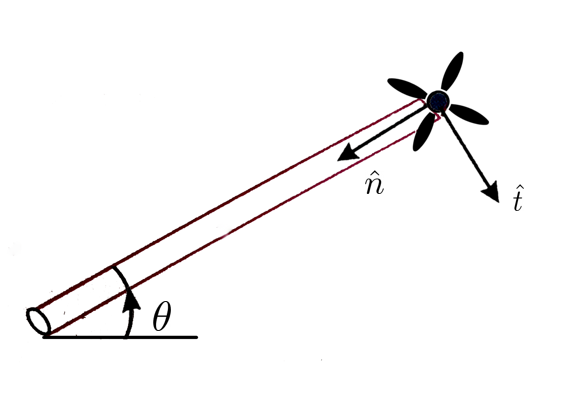
\includegraphics[width=0.8\textwidth]{./Imagenes/y_el_trozzo.png}
    \caption{Diagrama de la planta.}
    \label{fig:Sys}
\end{figure}

Se plantea el versor tangencial:
\begin{equation}
    \hat{t}: \\ mg\cdot \cos{(\theta)}=\frac{\partial P}{\partial t}
         \end{equation}
     
     \begin{equation}
    mg\cdot \cos{(\theta)}=v\cdot \frac{\partial m}{\partial t} + m \frac{\partial v}{\partial t}
         \end{equation}
     
     \begin{equation}
     mg\cdot \cos{(\theta)}-v\cdot \frac{\partial m}{\partial t} = m\cdot a
     \end{equation}
     
     \begin{equation}
     mg\cdot \cos{(\theta)}-\left( v_t - v_f\right)^2 \cdot \frac{\rho C_d A}{2}=m\cdot a\\
\end{equation}
Donde $\rho$ es la densidad del fluido, en este caso del aire, $C_d$ es el coeficiente de arrastre, $A$ es el área por la cual atraviesa el flujo de aire, $v_t$ es la velocidad tangencial del ventilador respecto de la mesa, y $v_f$ es la velocidad del aire expulsado gracias la rotación de las aspas.\\
Además sabiendo las siguientes relaciones:
\begin{equation}
    v_t=R\cdot \omega \ \ \ \ \ \ \ \ v_f = R_f\cdot \omega_f(t) \ \ \ \ \ \ \ \ \omega \cdot R = \dot{\theta} \ \ \ \ \ \ \ \  \alpha\cdot R = \ddot{\theta}
\end{equation}
Donde $R$ es el radio desde el pivote al ventilador, y $R_f$ el radio de las aspas, $\omega_f$ es la función de giro del ventilador.
\begin{equation}
     mg\cdot \cos{(\theta)}-\left( R\cdot \dot{\theta} - R_f \cdot \omega_f\right)^2 \cdot \frac{\rho C_d A}{2}=mR\cdot \ddot{\theta}\\
\end{equation}
Aquí se llega a una expresión del sistema, en el cual debido a la elección de actuador y sensor, se obtiene $\omega_f$ el cual será modificada por el actuador, y $\theta$ el cual es medido por el sensor.\\
Si se toman las siguientes aproximaciones:
\begin{equation} 
\left( R\cdot \dot{\theta} - R_f\cdot \omega_f \right)^2 \approx R\cdot \dot{\theta} - R_f\cdot \omega_f \ \ \ \ \ \ \ \ \cos{(\theta)}\approx \frac{\sqrt{2}}{2}
\end{equation}
se puede aproximar de la siguiente manera.

\begin{huge}
\begin{center}
	$\stackrel{\mathcal{L}}{\approx}$
\end{center}
\end{huge}

\begin{equation}
mg\frac{\sqrt{2}}{2} \delta(s) - \left( R\cdot s\theta(s) - R_f \omega_f(s) \right)\cdot \frac{\rho C_d A}{2} = m\cdot s^2\theta(s)   
\end{equation}
Aqui se puede apreciar que se puede estimar una transferencia lineal si se ignora el término gravitatorio, el cual tendrá 2 polos. Donde $\theta$ es la salida y $\omega_f$ es la entrada

\section{Implementación}

La arquitectura de control utilizada se observa en la Figura (\ref{fig:controlsys}).

\begin{figure}[H]
    \centering
    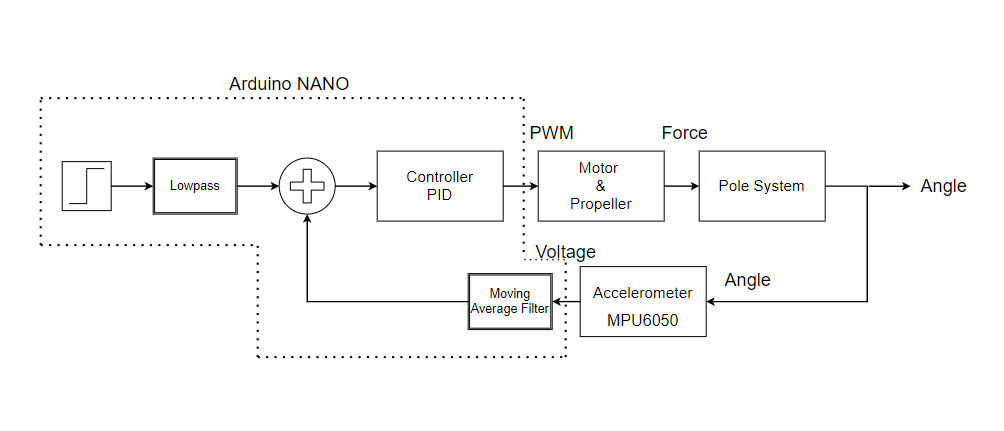
\includegraphics[width=\textwidth]{./Imagenes/controlsystem.png}
    \caption{Diagrama del sistema de control.}
    \label{fig:controlsys}
\end{figure}


Mientras que el hardware se conectó según la Figura (\ref{fig:hardwaresys}).

\begin{figure}[H]
    \centering
    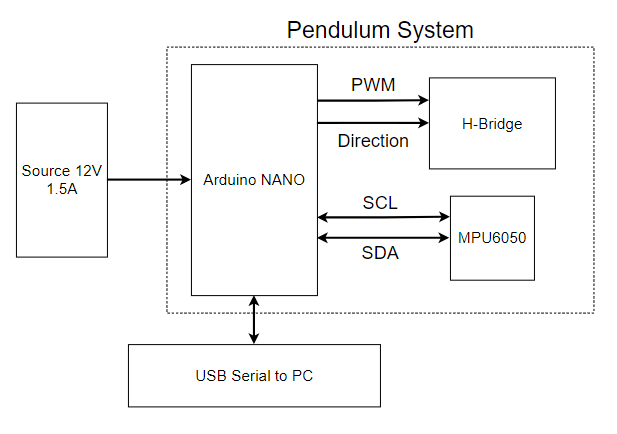
\includegraphics[width=0.8\textwidth]{./Imagenes/hardwaresystem.png}
    \caption{Diagrama del conexionado de hardware.}
    \label{fig:hardwaresys}
\end{figure}

Como punto de partida, se midió la respuesta del sistema a lazo cerrado con baja ganancia, observando que este se estabilizaba en cierto punto, pero con un error permanente grande. 

\begin{figure}[H]
    \centering
    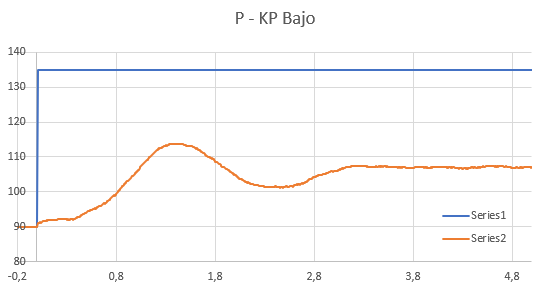
\includegraphics[width=0.8\textwidth]{./Imagenes/kplow.png}
    \caption{Respuesta al escalón del controlador proporcional. Setpoint en curva azul y ángulo en curva naranja.}
    \label{fig:kplow}
\end{figure}

Si bien este sistema se estabilizaba frente a una respuesta al escalón, frente a un disturbio se tornaba inestable como se observa en la Figura (\ref{fig:kpdist}).

\begin{figure}[H]
    \centering
    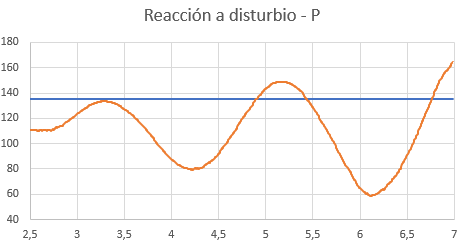
\includegraphics[width=0.8\textwidth]{./Imagenes/kpdist.png}
    \caption{Respuesta a disturbio del controlador proporcional. Setpoint en curva azul y ángulo en curva naranja.}
    \label{fig:kpdist}
\end{figure}

Por esto, se agregó control derivativo para estabilizar al sistema frente disturbios. Esto exageró significativamente el ruido del acelerómetro debido a que las vibraciones inducidas por el motor producían ruido que tras pasar por el derivador provocaban más vibraciones en el motor. Para reducir este efecto, se utilizó un filtro de media móvil. Con esto, el sistema se tornó estable frente a disturbios.

\begin{figure}[H]
    \centering
    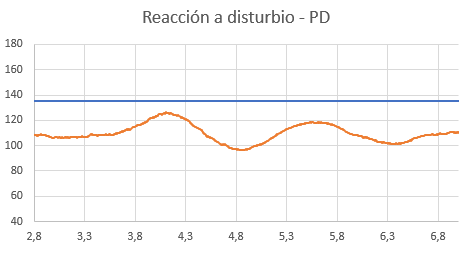
\includegraphics[width=0.8\textwidth]{./Imagenes/kddist.png}
    \caption{Respuesta a disturbio del controlador proporcional derivativo. Setpoint en curva azul y ángulo en curva naranja.}
    \label{fig:kddist}
\end{figure}

Sin embargo, el sistema aún poseía gran error permanente. Se agregó control integral con anti-windup para mitigar el error permanente quedando así la respuesta como se observa en la Figura (\ref{fig:ki}).

\begin{figure}[H]
    \centering
    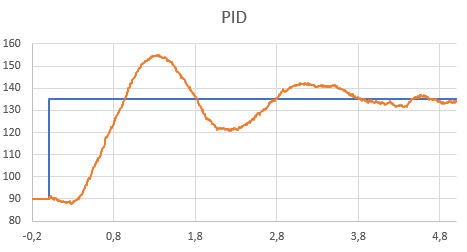
\includegraphics[width=0.8\textwidth]{./Imagenes/ki.png}
    \caption{Respuesta al escalón del controlador PID. Setpoint en curva azul y ángulo en curva naranja.}
    \label{fig:ki}
\end{figure}

Esta respuesta era demasiado oscilatoria, por lo que se colocó un prefiltro lo cual arregló este problema.

\begin{figure}[H]
    \centering
    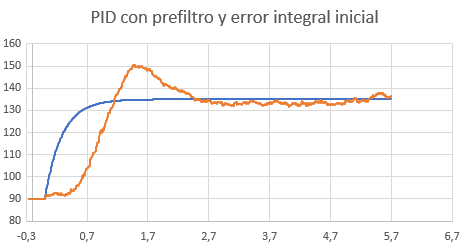
\includegraphics[width=0.8\textwidth]{./Imagenes/pidcompleto.png}
    \caption{Respuesta al escalón del controlador PID con prefiltro. Setpoint en curva azul y ángulo en curva naranja.}
    \label{fig:pidcompleto}
\end{figure}

Quedando así finalmente la respuesta frente a un disturbio como se observa en la Figura (\ref{fig:piddist}).

\begin{figure}[H]
    \centering
    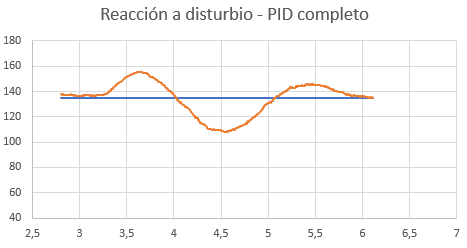
\includegraphics[width=0.8\textwidth]{./Imagenes/piddist.png}
    \caption{Respuesta a disturbio del controlador PID con prefiltro. Setpoint en curva azul y ángulo en curva naranja.}
    \label{fig:piddist}
\end{figure}

Finalmente, en las Figuras (\ref{fig:comptrans}) y (\ref{fig:compdist}) se puede observar una comparación entre las respuestas al escalón y las respuestas a disturbios.

\begin{figure}[H]
    \centering
    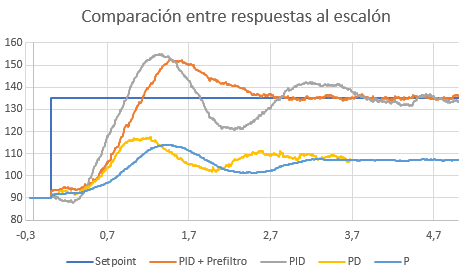
\includegraphics[width=0.8\textwidth]{./Imagenes/comptrans.png}
    \caption{Comparación entre las respuestas al escalón de los distintos controladores.}
    \label{fig:comptrans}
\end{figure}

\begin{figure}[H]
    \centering
    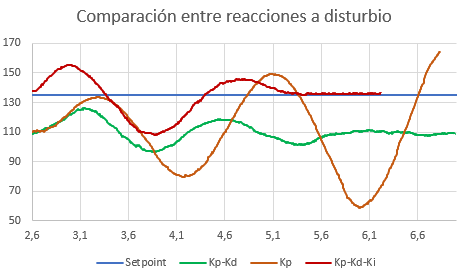
\includegraphics[width=0.8\textwidth]{./Imagenes/compdist.png}
    \caption{Comparación entre las respuestas a disturbio de los distintos controladores.}
    \label{fig:compdist}
\end{figure}

Finalmente, los valores de las sensibilidades quedaron $Kp = 0.55$, $Ki = 3\cdot dt$ y $Kd = \frac{0.45}{dt}$ ajustados a frecuencia de sampleo genérica. Para el prefiltro se utilizó un filtro IIR de primer orden con frecuencia de corte de $65Hz$. El filtro de media móvil es de 40 samples.

\section{Código}
Luego se presenta el codigo implementador para realizar el control:
    \lstinputlisting[language=C]{main.cpp}

\end{document}